\begin{figure}[htbp]
\centering
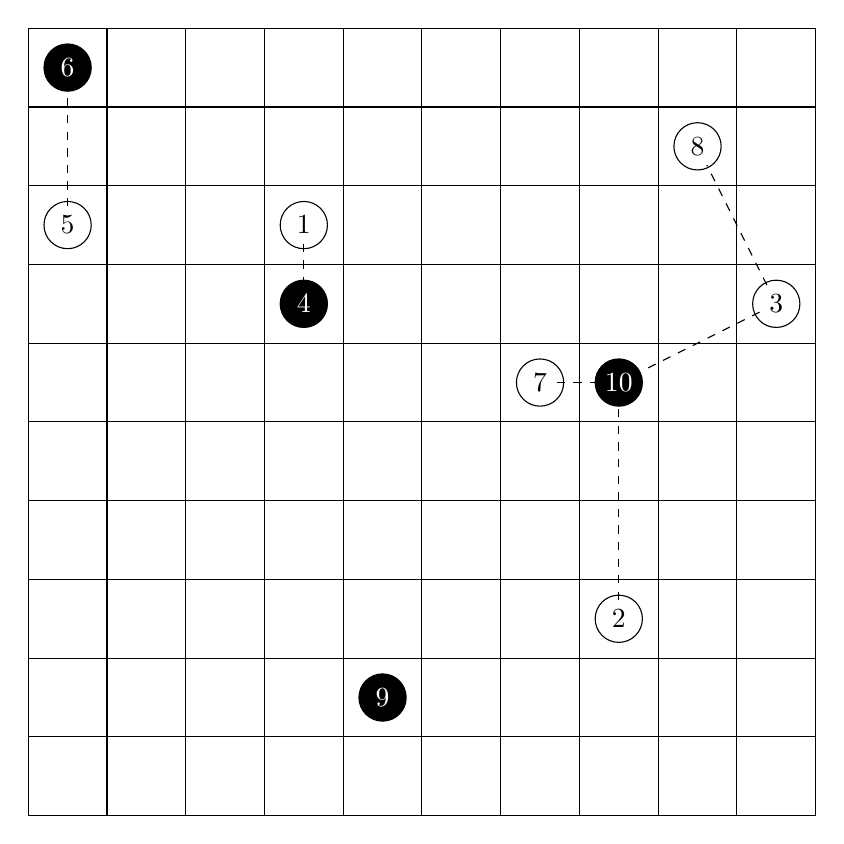
\begin{tikzpicture}

	\draw[xshift=0.5cm, yshift=0.5cm] (0,0) grid (10,10);
	\draw (4,8) circle [radius=0.3];
	\draw (8,3) circle [radius=0.3];
	\draw (10, 7) circle [radius=0.3];
	\draw[fill=black] (4, 7)  circle [radius=0.3];
	\draw (1, 8)  circle [radius=0.3];
	\draw[fill=black] (1, 10) circle [radius=0.3];
	\draw (7, 6)  circle [radius=0.3];
	\draw (9, 9)  circle [radius=0.3];
	\draw[fill=black] (5, 2)  circle [radius=0.3];
	\draw[fill=black] (8, 6)  circle [radius=0.3];

	\draw node (v1) at (4,8) {1};
	\draw node (v2) at (8,3) {2};
	\draw node (v3) at (10, 7) {3};
	\draw[white] node (v4) at (4, 7)  {4};
	\draw node (v5) at (1, 8)  {5};
	\draw[white] node (v6) at (1, 10) {6};
	\draw node (v7) at (7, 6)  {7};
	\draw node (v8) at (9, 9)  {8};
	\draw[white] node (v9) at (5, 2)  {9};
	\draw[white] node (v10) at (8, 6)  {10};

	\draw[style=dashed] (v1) -- (v4);
	\draw[style=dashed] (v2) -- (v10);
	\draw[style=dashed] (v3) -- (v8);
	\draw[style=dashed] (v3) -- (v10);
	\draw[style=dashed] (v5) -- (v6);
	\draw[style=dashed] (v7) -- (v10);
	
\end{tikzpicture}

\emph{Se tienen 4 centrales disponibles}

\caption{Soluci\'on del problema de la Figura \ref{ej_2:aleatorio} dado por el algoritmo propuesto, con las 10 ciudades y las 4 centrales hubicadas en los nodos oscuros}
\label{ej_2:aleatorio:sol}
\end{figure}
